% !TeX root = ../main.tex
% Add the above to each chapter to make compiling the PDF easier in some editors.

\chapter{Implementation}\label{chapter:implementation}

The general work of the solution looks as following. The researcher creates \textit{config.xml} that contains the configurations of bookmarks and surveys (details in Subsection \ref{subsec:configuration}) and custom trigger classes (Subsection \ref{subsec:triggers}). They are used by the \textit{experiment} package that interacts with the \textit{workbench} code to make the changes in display and behavior and collect the data during the experiment. Therefore it generates media files: audio, webcam ans screen recordings and makes changes to the \textit{event.log}. Details can be found in Subsections \ref{subsec:recording} and \ref{subsec:logging} correspondingly. These files in a proper structure (see \ref{subsec:fileStructure} together with \textit{config.xml} are used by the Analysis Tool to provide the functionality described in Chapter \ref{chapter:approach}. The implementation of the Analysis Tool is described in Section \ref{section:analysisTool}.\\

\begin{figure}[htb]
 \centering
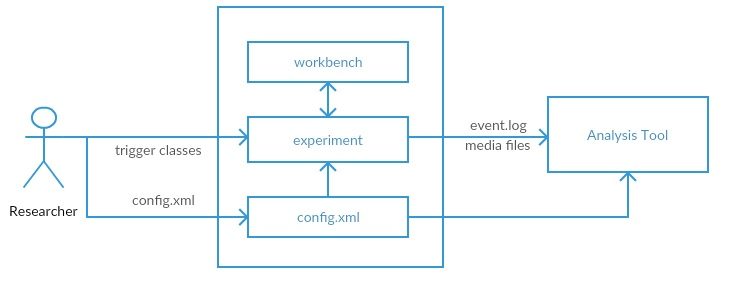
\includegraphics[width=\textwidth]{figures/arhitecture.jpg}
\caption{Solution architecture}
\label{fig:architecture}
\end{figure}


\section{Data collection}\label{section:dataCollectionIntegration}

Data collection is performed within workbench code. Most of the changes are the new classes inside the \textit{experiment} package, although there are other minor changes, for example in the \textit{MainController} to display buttons according to the Bookmarks configuration. The resulting class diagram of the \textit{experiment} package is on the Figure \ref{fig:data_collection_diagram_actual}.Media files are collected automatically at the start of the application. Details of how it's done can be found in Subsection \ref{subsec:recording}. \\

\begin{figure}[htb]
 \centering
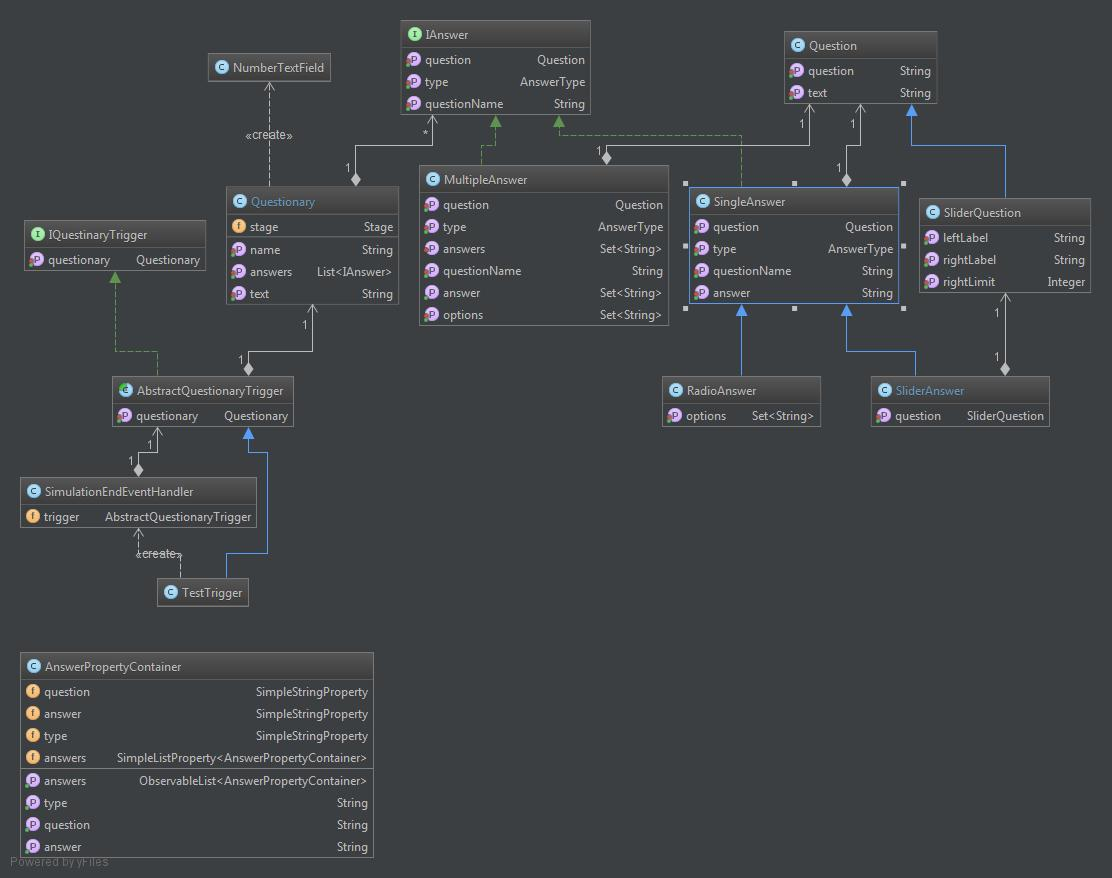
\includegraphics[width=\textwidth]{figures/diagram.jpg}
\caption{Class diagram of the \textit{experiment} package.}
\label{fig:data_collection_diagram_actual}
\end{figure}

Bookmarks are displayed as buttons and menu items in the top toolbar of the workbench (See Figure \ref{fig:panel}). Bookmarks can be augmented with icons to display in the button/menu item. Time Interval bookmarks distinct from Timepoint bookmarks by having a state in the text of a button/menu item. The initial state of the element is "stopped" therefore it is displayed as "Name (Start)", so the user knows he starts the activity by clicking the button. Click toggles the state of the Bookmark and it's displayed as "Name (Stop)". The state can be changed multiple times, on the case of repeatable activity or participant's mistake.\\

The Survey is displayed in a popup window. It can be called either by the user clicking a Bookmark or a custom trigger designed by the researcher. A click on the "Save" button in the Survey window saves the results in the log file. The entries of the user answer are saved in the Survey form, thus if the user has closed the window by a mistake, he doesn't have to reenter all the answers when he reopens the survey window.\\



\begin{figure}[htb]
 \centering
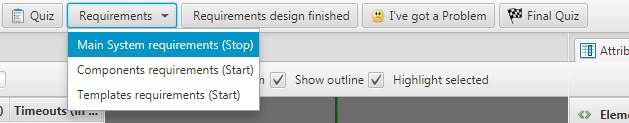
\includegraphics[width=\textwidth]{figures/panel.jpg}
\caption{Bookmarks as buttons and menu items}
\label{fig:panel}
\end{figure}



\subsection{Configuration}\label{subsec:configuration}
Configuration of the Boormarks and Surveys is done in the \textit{config.xml} file. The structure is as following:

\lstset{
  language=XML,
  showstringspaces=false,
}
\begin{lstlisting}
<events>
    <event name="Quiz" icon-name="tasks.png">
        <questionary name="Quiz" text="Please answer the questions">
            <question type="number" name="age" text="How old are you?"></question>
            <question type="checkbox" name="background"...>
            <question type="radio" name="mecExperience"...>          
            <question type="radio" name="mecSoftwareExperience"...>
            <question type="radio" name="reqExperience"...>
            <question type="radio" name="userStudyExperience"
                      text="Have you ever participated in User Studies">
                <radio text="Yes"></radio>
                <radio text="No"></radio>
            </question>
        </questionary>
    </event>
    <event-group name="Requirements">
        <event name="Main System requirements" range="true" on-start="false"...>
        <event name="Components requirements" range="true" on-start="false"...>
        <event name="Templates requirements" range="true" on-start="false"...>
    </event-group>
    <event name="Requirements design finished"...>
    <event name="I've got a Problem" icon-name="face-sad.png"...>
    <event name="Final Quiz" icon-name="finish_flag.png"...>
    <trigger className="de.tum.imomesa.workbench.experiment.TestTrigger">
        <questionary text="Simulation was done" name="simulation"...>
    </trigger>
</events>

\end{lstlisting}

Bookmarks are defined with element \textit{event}. It has a name, that has to be unique and might name an \textit{icon-name} that specifies a name of an icon in the \textit{resources/icons/events} folder. Events under the \textit{events} root element are displayed as buttons. Events can be grouped into \textit{event-group} element to be displayed as menu items. The name of the \textit{event-group} is the name of the menu.   In order to specify a Time Interval, attribute \textit{range} has to be set to \textit{true} and \textit{on-start} attribute shows whether the Survey is triggered at the beginning or end if the interval. Surveys are defined with \textit{questionary} element. Besides of the unique \textit{name} attribute it has a \textit{text} attribute that defines the label of the Survey.\\

Questions are configured with \textit{question} element and the type of the question is defined by the \textit{type} attribute. Type can be one of the following:
\begin{itemize}
\item \textit{checkbox} for a Multiple choice question
\item \textit{radio} for a Single Choice question
\item \textit{text} for a Free Form feedback
\item \textit{number} for a Number question
\item \textit{slider} for a Liker Scale
\end{itemize}
Chexkbox and Radio Questions require options configured with \textit{checkbox} and \textit{radio} elements under the \textit{question} element. The options have a \textit{text} attribute that is displayed as the label of checkbox/radiobutton.\\

Triggers have an attribute \textit{className} that defines the name of the class that implements the trigger functionality. Trigger can have a \textit{questionary} child element to define the Survey the Trigger calls. Details about the implementation of the Trigges classes can be found in Subsection \ref{subsec:triggers}\\

\subsection{Custom event triggers} \label{subsec:triggers}

The Trigger class has to implement the \textit{IQuestionaryTrigger} interface, which is presented below. The Trigger has to implement the custom functionality in the \textit{init} method. It is supposed that there is some listener initialization in the \textit{init} method, but it's up to the researcher.\\  

\lstset{language=Java} 
\begin{lstlisting}
public interface IQuestinaryTrigger {
    void init();
    void callQuestionary();
    void setQuestionary(Questionary questionary);
    Questionary getQuestionary();
}
\end{lstlisting}

There is an abstract class called \textit{AbstractQuestionaryTrigger} that implements the Survey related functionality. Usually the Trigger has a Survey, so this abstract class implements getter, setter and displays the  Survey in \textit{callQuestionary} method.\\


\lstset{language=Java} 
\begin{lstlisting}
public abstract class AbstractQuestionaryTrigger implements IQuestinaryTrigger {
    public Questionary getQuestionary() {
        return questionary;
    }
    public void setQuestionary(Questionary questionary) {
        this.questionary = questionary;
    }
    private Questionary questionary;
    @Override
    public void callQuestionary() {
        questionary.show();
    }
}
\end{lstlisting}

Below you can see an example of a custom trigger class that calls the Survey after the \textit{SimulationEndEvent} happens. This Trigger is used to collect the fresh impression of a participant about the results of the simulation. As you can see the class implements the \textit{init} method, where there is a listener is subscribed to the \textit{EventBus}. For this example an additional class \textit{SimulationEndEventHandler} to handle the event and display the Survey.\\

\lstset{language=Java} 
\begin{lstlisting}
public class TestTrigger extends AbstractQuestionaryTrigger {
    @Override
    public void init() {
        EventBus.getInstance().subscribe(new SimulationEndEventHandler(this));
    }
}

public class SimulationEndEventHandler implements EventHandler {
    AbstractQuestionaryTrigger trigger;

    public SimulationEndEventHandler(AbstractQuestionaryTrigger trigger){
        this.trigger = trigger;
    }
    public void handle(SimulationEndEvent event){
        trigger.callQuestionary();
    }
}
\end{lstlisting}

Triggers don't have to use the \textit{EventBus}. The researcher can put any functionality into the class, for example the researcher might configure a Timer to call the Survey every 15 minutes. \\

% The Triggers also don't have to call a Survey. For example, if the researcher wants the participants to follow the Pomodoro Technique, he can configure a 25 minutes timer and displaying a window in \textit{callQuestionary} method.

\subsection{Media files recording} \label{subsec:recording}
Media files recording uses classes from the \textit{tracker/recorders} package to generate three files: two .mov files for the screen and webcam recordings and one .wav file for the microphone recording. The files are saved into the \textit{temp} folder in the workbench directory.\\

\subsection{Logging}\label{subsec:logging}

We use the inner event logger of the  workbench to save the Bookmark and Survey data. \textit{QuestionarySubmitEvent} is used to save the JSONObject with the data into the log file. The file is stored in the run folder of the workbench.\\
\lstset{language=Java} 
\begin{lstlisting}
public class QuestionarySubmitEvent extends Event {
    public Object getAnswers() {  return answers.get();   }
    public ListProperty answersProperty() {        return answers;    }
    private ListProperty answers = new SimpleListProperty<AnswerPropertyContainer>();
    public String getQuestionaryName() {        return questionaryName.get();    }
    public StringProperty questionaryNameProperty() {        return questionaryName;    }
    private StringProperty questionaryName = new SimpleStringProperty();

    public QuestionarySubmitEvent(Questionary questionary) {
        List<IAnswer> questionaryAnswers = questionary.getAnswers();
        ArrayList<AnswerPropertyContainer> answerPropertyContainers = new ArrayList<>();
        for (IAnswer answer : questionaryAnswers) {
            AnswerPropertyContainer answerPropertyContainer;
            if(answer.getType()== IAnswer.AnswerType.Checkbox){
                MultipleAnswer multipleAnswer = (MultipleAnswer)answer;
                answerPropertyContainer = new AnswerPropertyContainer(answer.getQuestionName(),
                        multipleAnswer.getAnswer(), answer.getType().name());
            }else{
                SingleAnswer singleAnswer = (SingleAnswer) answer;
                answerPropertyContainer = new AnswerPropertyContainer(answer.getQuestionName(),
                        singleAnswer.getAnswer(), answer.getType().name());
            }
            answerPropertyContainers.add(answerPropertyContainer);
        }
        answers.set(FXCollections.observableArrayList(answerPropertyContainers));
        questionaryName.set(questionary.getName());
    }
}
\end{lstlisting}

\section{Analysis Tool}\label{section:analysisTool}

In this section we present the file structure of the files collected during the experiment and the implementation of three main functional modules of the Analysis Tool: Overview, Statistics and Text answers as well as general aspects of functionality of the Analysis Tool.\\ 

\subsection{General functionality}

As input the Analysis Tool accepts the files form the experiments. The tool is designed to work not only with one experiment, but with multiple experiments. For convenience the session are grouped by the workstation, so if the participant turns the station off and on or the experiment takes more then one session, the sessions are grouped logically. The grouping of the sessions data into according to the workstation is the responsibility of the researcher. The researcher has to collect the data from the workstations and put them into the directory of the Analysis Tool in the proper structure. \\

The main data entities the tool works with are \textit{Sessions} and \textit{SessionGroups}, that contain \textit{Sessions} (See Figure \ref{fig:session_sg}). The \textit{SessionGroups} are supposed to represent the sessions performed on one workstation or by one person, but it's up to the researcher to use the grouping of the sessions as he prefers. The sessions are grouped according to the folders.\\

\begin{figure}[htb]
 \centering
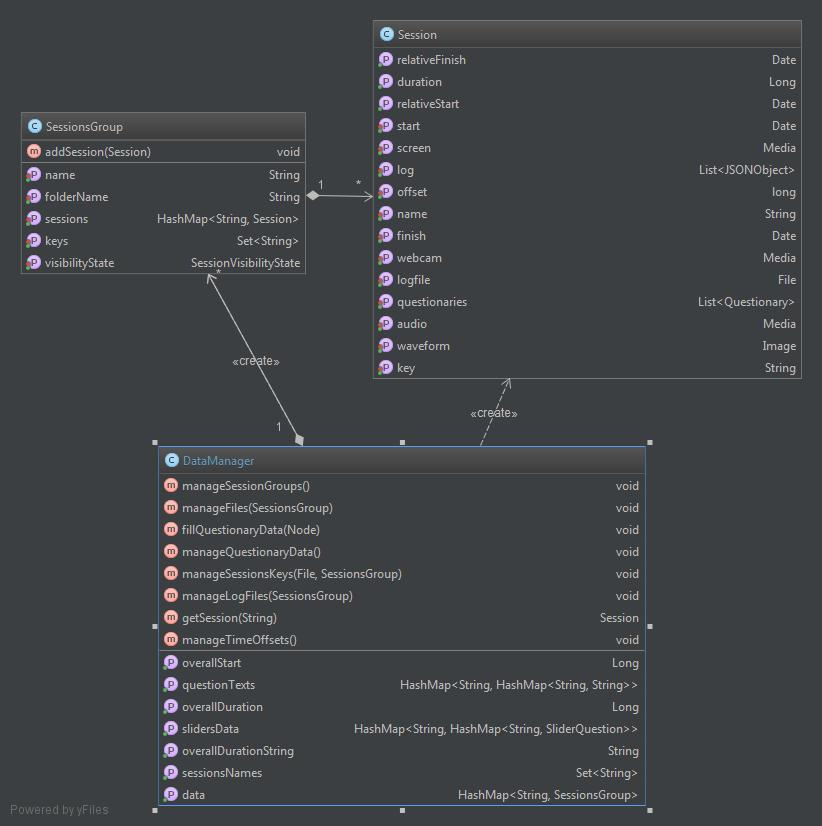
\includegraphics[width=340pt]{figures/session_sg.jpg}
\caption{Session, SessionGroup, DataManager}
\label{fig:session_sg}
\end{figure}

\textit{Session} class contains all session data collected during the experiment. \textit{DataManager} is a singleton class that provides the data access for all the tool. It reads the files from the filesystem, parses the logfiles and generates the proper structure of \textit{SessionGroups} and \textit{Sessions} with filled fields. It also provides other functionality needed for the modules, like offset management (Details in \ref{subsec:overview}).\\

The \textit{Context} class is a singleton accessed by controllers to share such common properties as screen mode and highlighted session id. As the tool works in two modes: window and fullscreen, the \textit{Context} is used for the controllers to display the content according to the mode. Highlighted session is shared by \textit{Statstics} and \textit{Text Answers} tabs, so the researcher keeps the session highlighted during the navigation between tabs.\\

\textit{CategoriesColors} is a class that provides the set of colors used as categories colors in different parts of the tool, for example for Surveys, Bookmarks, Questions. It's a singleton, that contains the set of hardcoded colors and a function to get a color. \textit{Constants} class contains constants used by different parts of the code, for example default window width. \\

The views are defined in the \textit{views} package. \textit{Main.fxml} defines the general view of the application: form, header, left navigation pane ans settings pane. Other three views (see Figure \ref{fig:views}) describe the views of the corresponding tabs. The functionality of navigation and window mode change is in the \textit{Main} controller. The styles are defined in the \textit{styles} package.\\

\begin{figure}[htb]
 \centering
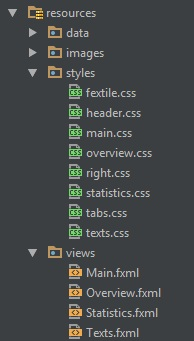
\includegraphics[width=110pt]{figures/views.jpg}
\caption{Styles ans views}
\label{fig:views}
\end{figure}

\subsection{File structure}\label{subsec:fileStructure}
The researcher is supposed to create a folder for every workstation. The name of the folder should be as following "sessions\textunderscore<workstation name>". This name will be displayed in the Analysis Tool. It is supposed that all three media files are present in the folder. There is no need to divide the log file, if one log file contains the log data from several session. The name of the log file is irrelevant, although names of the media files should not be changed - they contain the key of the session.\\

\subsection{Overview}\label{subsec:overview}

The task of the Overview tab is to display the media files of the sessions, waveforms of the audio files, a bookmark timeline that shows timepoints and time intervals and displays a survey result attached to the bookmark. It also has to provide the functionality to hide/show the bookmarks according to the type and hide/show/expand/collapse the video files and mute/unmute the audio. There is a common timeline that controls all the sessions, so they would play simultaneously. The control over the timeline has to be done either via the timeline slider, either by clicking on the waveform panel. There is a vertical line that shows the current time(see Figure \ref{fig:overview_3}). The time is always synchronized for all sessions.\\

\begin{figure}[htb]
 \centering
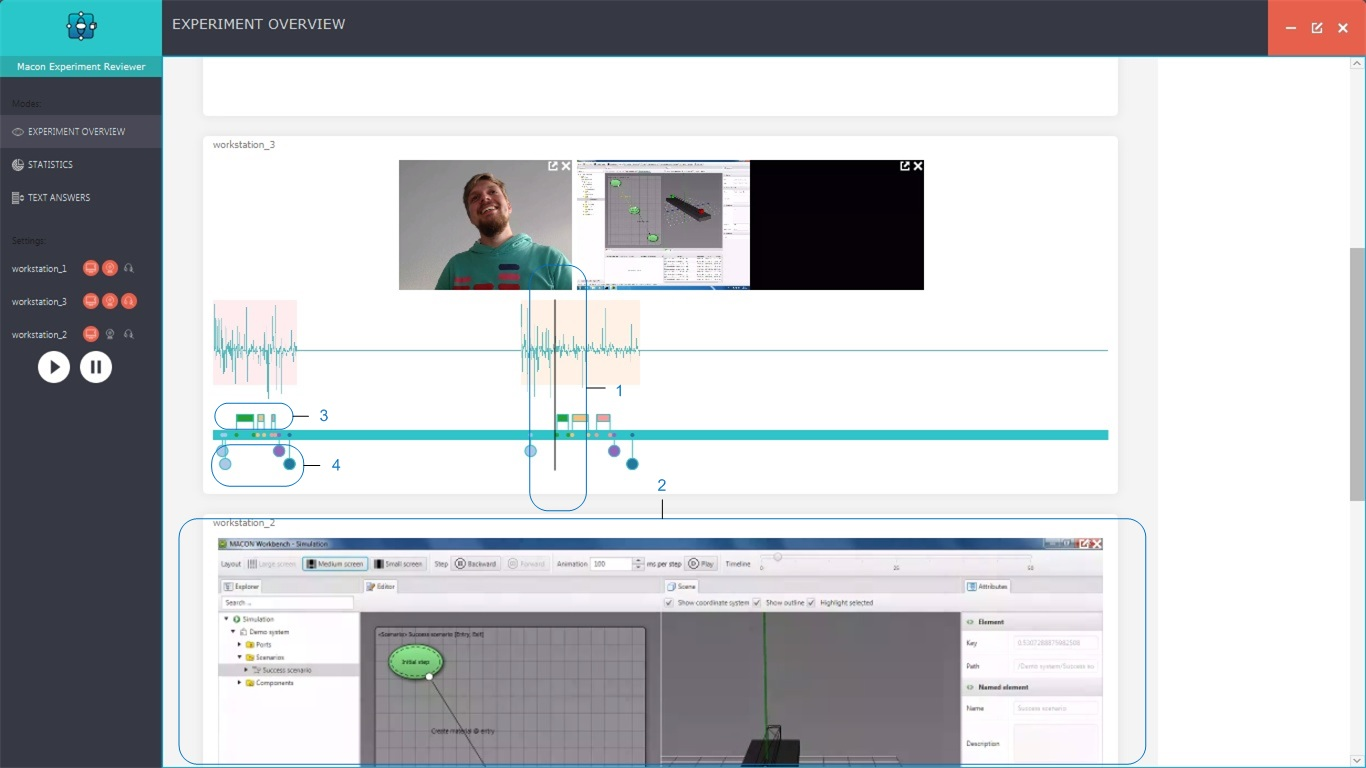
\includegraphics[width=\textwidth]{figures/overview_3.jpg}
\caption{Overview tab. 1 - line of the current playing time, 2 - expanded screen video, 3 - time intervals, 4 - timepionts.}
\label{fig:overview_3}
\end{figure}

In order for the timeline not to be stretched by the gaps between the sessions, the gaps are being removed. The original time of the sessions is stored in the \textit{Session} class, while the sessions are processed in the \textit{DataManager}, the offsets are computed for the sessions to generate the relative time in order to get a consistent timeline. The logic of the offsets management is on the Figure \ref{fig:offsets_management}.\\

\begin{figure}[htb]
 \centering
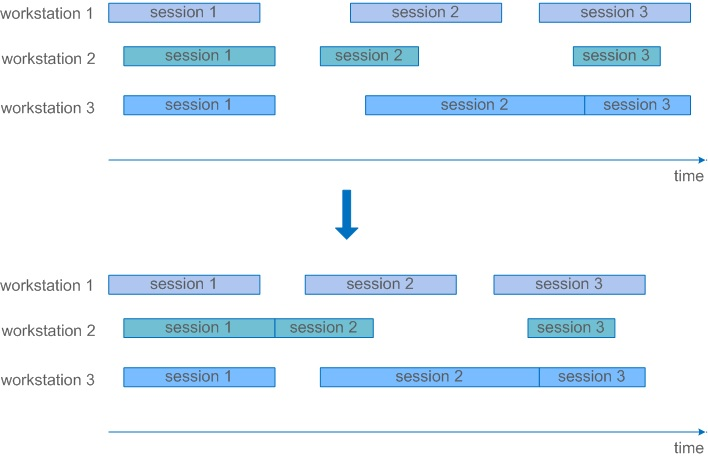
\includegraphics[width=300pt]{figures/offsets_management.jpg}
\caption{Sessions time offsets management}
\label{fig:offsets_management}
\end{figure}

The class diagrams of most of the classes that are used to fulfill the functionality is presented in Figure \ref{fig:d1}. \textit{Overview} controller is the controller of the tab. It creates the instance of the \textit{TimelineController} that created the timeline and   \textit{SessionGroupContainers} and places them into the view.\\

\begin{figure}[htb]
 \centering
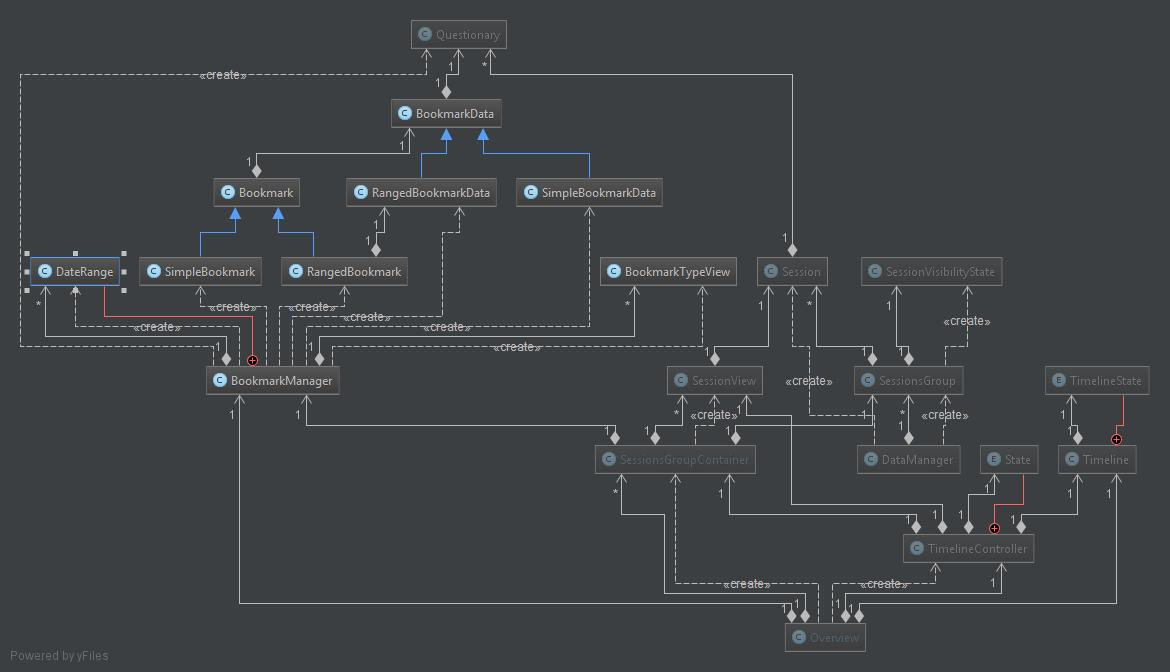
\includegraphics[width=\textwidth]{figures/diagram1.jpg}
\caption{Class diagram of the \textit{overview} package}
\label{fig:d1}
\end{figure}

\textit{SessionView} contains the MediaPlayers of the media files of the \textit{Session} and the ImageView of the waveform. The image of the waveform is created by the \textit{AudioWaveformCreator} class. The \textit{SessionGroupContainer} is in charge for the display of a \textit{SessionGroup}, including media players of a proper session, offset of the waveform, bookmarks pane, implementation of play, pause, seek functions, that include the selection of the session according to the time. \textit{SessionGroupContainer} also implements the functionality of hiding/showing/expading/collapsing screen and webcam players, muting/unmuting the audio. The \textit{Overview} controller also fills the settings pane with the list of session groups and icons to toggle the visibility or mute the session group. The controller is subscribed to the \textit{seekProperty} of the \textit{SessionGroupContainer} to respond on the click on the waveform container that has to result in the playing time change. \textit{SessionGroupContainer} has a method to update the vertical line position and \textit{Overview} controller calls this method when the global time property is being changed. \\

\textit{TimelineController} manages the timeline and calls the seek, play and pause methods of the containers. \textit{TimelineController} always has at least one playing session and uses one of them as an active session that updates the timeline. \textit{TimelineController} has a logic to detect the situation, when the active session is over and there is a need to set a different session as the active playing session. The logic of selecting a session (or no session) to play according to the time is in the \textit{SessionGroupContainer}.\\

The Bookmarks for the bookmarks timeline are generated by the \textit{BookmarkManager} which is a singleton and processes the data from the \textit{DataManager} to generate the visual bookmarks for every session. The bookmarks are of two types: timepoint and time interval and are visualized by different items in the bookmark pane (See Figure \ref{fig:overview_3}). The toggling of visible/invisible state of the bookmarks is also implemented in the \textit{BookmarkManager}. \\



\subsection{Statistics}
Statistics tab is a dashboard that shows the results of the Surveys. The class diagram of most of the classes involved in the functionality of the statistics tab is on the Figure \ref{fig:d2}. \textit{StatisticsItemsManager} is a singleton that goes through the data in \textit{DataManager} and forms the list of \textit{StatisticsItemsContainers} which is basically a representation of results of one Survey. The \textit{Statistics} controller forms the Survey pane, which is a list of Surveys, where the user can toggle the visibility of the Survey container and a displays a container for every visible \textit{StatisticsItemsContainer}. The controller fills the settings pane with the list of sessions grouped by session groups with an icon for highlighting.\\

\begin{figure}[htb]
 \centering
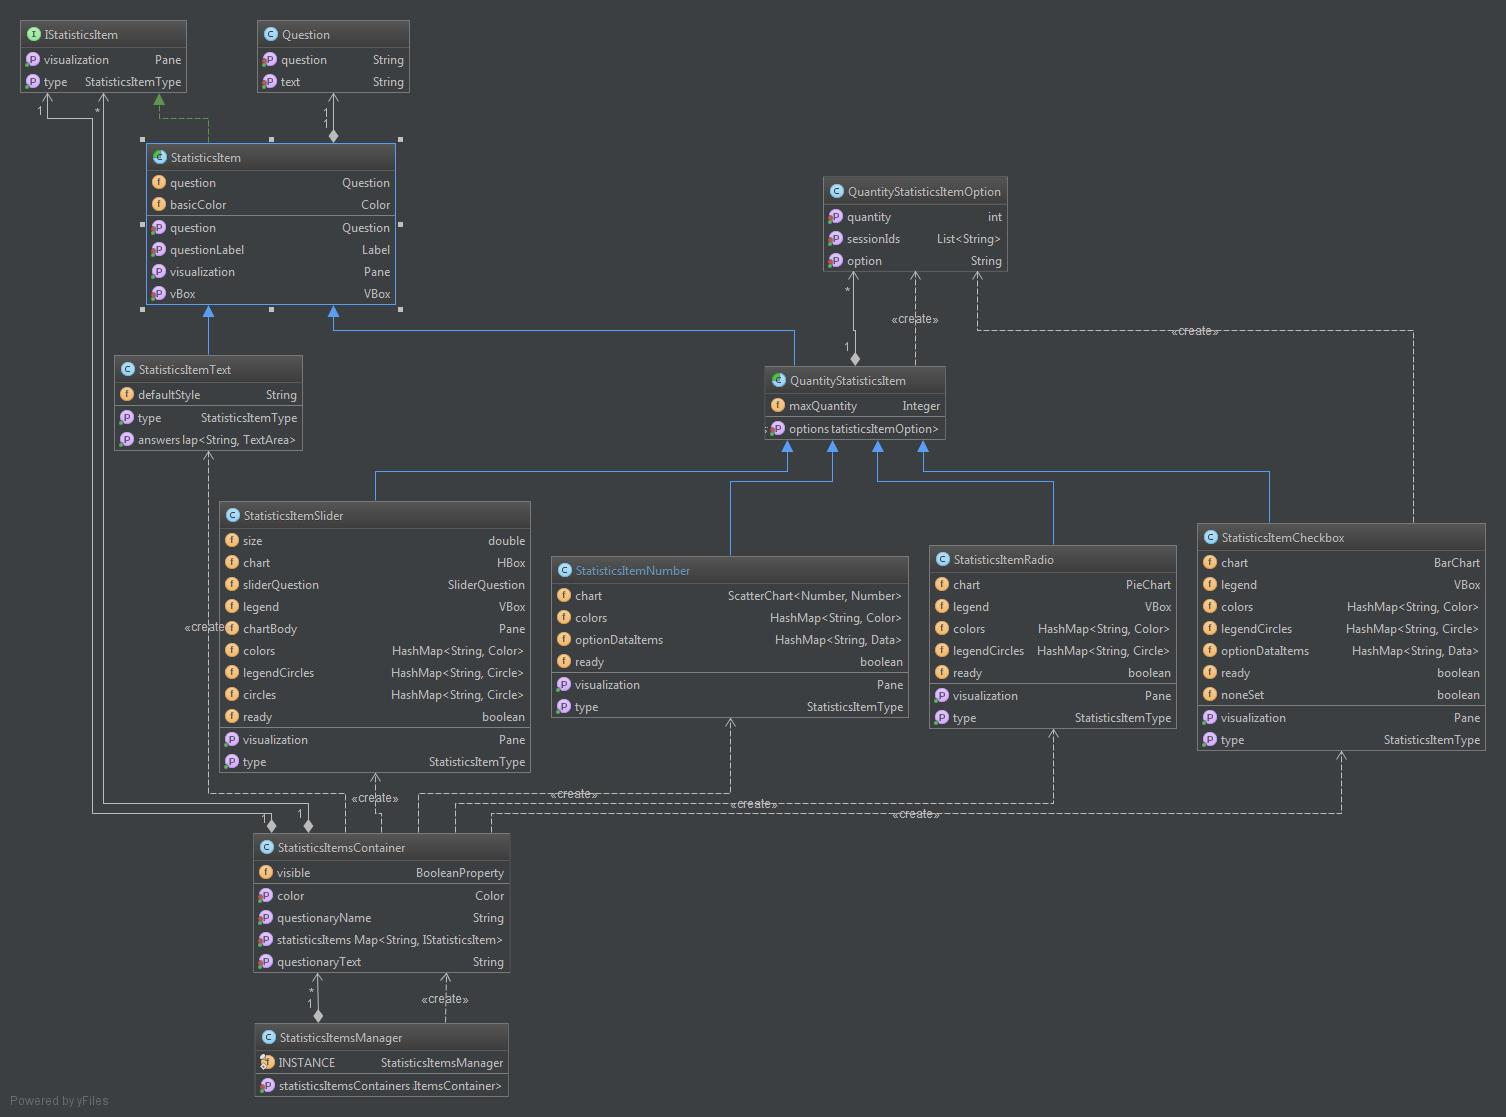
\includegraphics[width=\textwidth]{figures/diagram2.jpg}
\caption{Class diagram of the \textit{statistics} package}
\label{fig:d2}
\end{figure}

\textit{StatisticsItemsManager} goes through the data and forms the list of \textit{IStatisticsItem}, which is a general interface of a statistics item.\\


\lstset{language=Java} 
\begin{lstlisting}
public interface IStatisticsItem {
    enum StatisticsItemType {
        Text, Slider, Radio, Checkbox, Number
    }
    Pane getVisualization();
    void highlight(String sessionKey);
    void addAnswer(String sessionId, IAnswer answer);
    void resize(Double columnWidth);
    void init(String sessionId, Question question, IAnswer firstAnswer, Color color);
    StatisticsItemType getType();
}
\end{lstlisting}

The statistics item is basically the representation of the answers to one question and it is supposed to provide a visualization, respond to the window size change, highlight the answer(or category that includes the answer) of the selected session, be initialized with the basic color of the Survey and the Question and allow to add an answer to the set of answers. Abstract class \textit{StatisticsItem} provides the general functionality of a statistics item, like displaying the question. \\

\textit{StatisticsItemConteiner} checks the type of the answer and creates the statistics item according to the type. \textit{StatisticsItemText} implements the \textit{IStatisticsItem} interface and displays a TextArea for every free form feedback answer. For every other type of answer the abstract class \textit{QuantityStatisticsItem} is used. It divides the answers into categories called options and computes the quantity of the answers in each category. \textit{StatisticsItemRadio, StatisticsItemCheckbox, StatisticsItemSlider and StatisticsItemNumber} extend the \textit{QuantityStatisticsItem} class and implement the visualization and highlighting.\\

\subsection{Text Answers}
Text Answers tab provides the functionality for the processing of the free form answers by labeling them and displaying the visualization. Figure \ref{fig:d4} shows the classes of the \textit{texts} package and some other classes that participate in the functionality.\\

\begin{figure}[htb]
 \centering
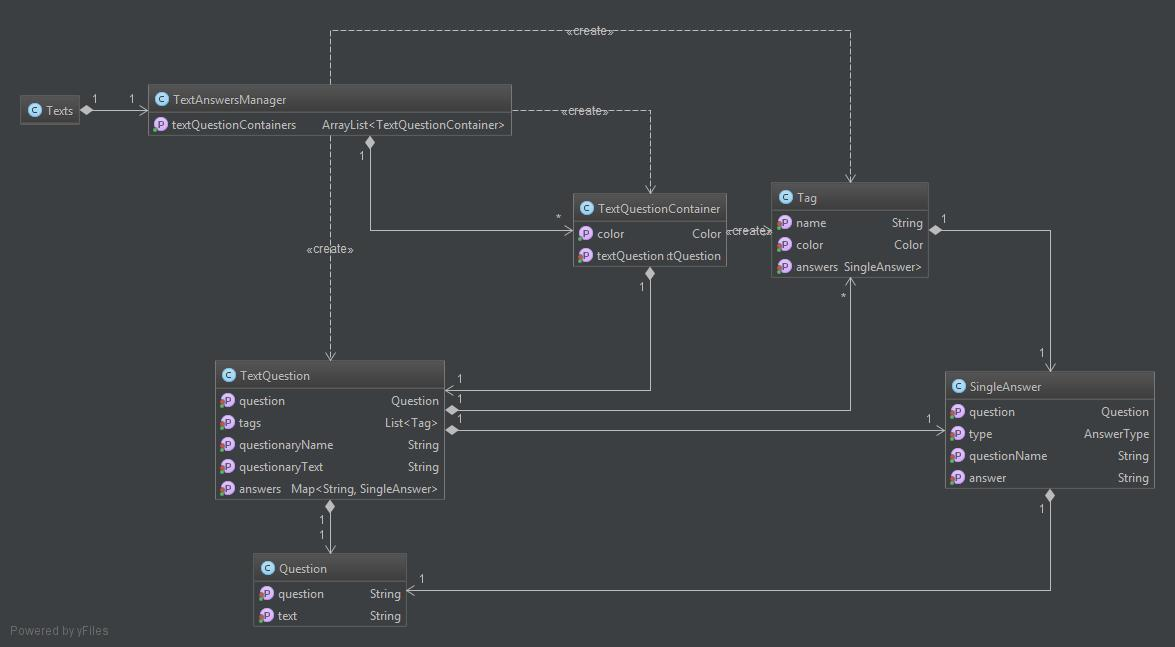
\includegraphics[width=\textwidth]{figures/diagram4.jpg}
\caption{Class diagram of the \textit{texts} package}
\label{fig:d4}
\end{figure}

The \textit{Tag} class represents the label the researcher can mark an answer with. A tag has a name, a color, and the set of marked answers. \textit{TextQuestionContainer} represents the visual container of a question, \textit{TextQuestion} represents the data behind the question, including list of \textit{Tags} and answers, name and label of the Survey. \textit{TextAnswerManager} is a singleton used by the \textit{Texts} controller, which manages the text question data and generates the containers, initial tags. Initially the manager iterates through the answers and generates a \textit{Tag} for every unique answer and marks the answer with the tag. If the answers are identical they are marked with the same tag.\\

The operations of editing, creation and deleting of labels as well as marking and unmarking the answer with labels is implemented in the \textit{TextQuestionContainer}. The behavior is based on listeners, so the visualization and the legend change immediately during changes, so the user doesn't waste the time of Save button ans sees the result instantly. The \textit{Texts} controller also fills the Question pane with the names of the free form questions grouped by Survey and allows to toggle visibility of the question.\\




